%!TEX root = rapport.tex

\chapter{Existing visualizations in lambda theory}

There does not exist anything similar to what we are doing in this thesis.
However, there does exist many examples of projects making other types of
visualizations of the lambda calculus. In this section we will discuss these.

There are numerous examples of software with which a lambda term or a
reduction step for a lambda term can be visualized. We have found 7 examples
of such programs. For a complete list, see Appendix \ref{app:a}.
What differentiates these examples from this project are mainly two things:
\begin{itemize}
	\item
	In our project we focus on the reduction graphs, and not on
	the particular reductions, whereas the earlier work focus on
	visualizing either particular reduction steps or the syntactic structure
	of lambda terms. 
	
	\item
	None of the existing visualizations are in our opinion very good-looking.
\end{itemize}

In the rest of this chapter we will describe the two most interesting examples.

\section{Alligator Eggs -- A Puzzle Game by Bret Victor}

% \begin{figure}[h!]
% 	% \centering
% 		
\includegraphics[width=0.1in]{../images/AlligatorEggs.png}
% 	\caption{Alligator Eggs -  A Puzzle Game}
% 	\label{fig:images_AlligatorEggs}
% \end{figure}

The ``Alligator Eggs - A Puzzle Game'' \cite{Alligator} is a ``fun'' and
children-like way of visualizing $\beta$-reductions of a lambda term. It was
originally not intended to be a computer program; the author instead designed
a set of drawings meant to be printed and cut out. This way, the visualization
can be used as a game. It visualizes the syntactic structure of lambda
terms, and the allowed ``moves'' in the game correspond to $\alpha$-conversion or
$\beta$-reduction.

The game uses a simple graphical alphabet:
\begin{description}
	\item[A hungry alligator] represents a lambda abstraction. The symbol can
	have different colors, analogously to variable names in ordinary lambda calculus.
	\item[An old alligator] is a parenthesis. It can only be white.
	\item[An egg] is a variable. It, too, can take on different colors.
\end{description}
Alligators are organized vertically into ``families''. The different families
are organized horizontally next to each other, and they are guarded by either an
old or a hungry alligator. The old alligator only concerns itself with
guarding, while the hungry alligator also has one or more eggs associated. If
an alligator and an egg are associated with each other, they have the same
color. It is straightforward to see the analogy to lambda terms.

With this alphabet, the rules are defined as follows:
\begin{description}
	\item[The Eating Rule] states that the topmost hungry alligator of a family can
	eat the family in front of it. When it does this it dies, but the eaten family
	is resurrected in its entirety from all the eggs associated with the hungry, dead
	alligator. This rule corresponds to a $\beta$-reduction. 
	\item[The Color Rule] states, that if an eaten family contains alligators and eggs
	in the same color as some alligators or eggs in the eating family, these must change colors
	to some new, unused color. This rule corresponds to an $\alpha$-conversion.
	\item[The Old Age Rule] states, that if the topmost alligator of a family is
	an old alligator, this alligator may die and nothing will happen. This is in analogy
	to the convention, that outermost parentheses in lambda terms are removed.
\end{description}

In figure \ref{fig:images_alligatorEat} we can see the Eating Rule in use. The
green alligator will eat whatever is in front of it. In this case it will eat
the yellow alligator and its yellow egg. After the green alligator has eaten
the yellow alligator and egg, it will die and its egg will hatch into what it
has eaten. ``The miracle of life'', as the author calls it. This so-called
``miracle'' is in our profane terminology called a $\beta$-reduction, as
mentioned above.

% \begin{figure}[htbp]
% 	\centering
% 		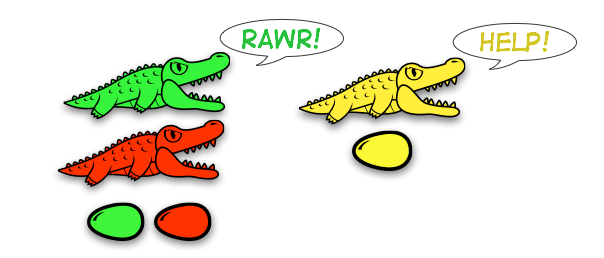
\includegraphics[width=2in]{../images/alligatorEat.png}
% 	\caption{A reduction visualized as an alligator eating}
% 	\label{fig:images_alligatorEat}
% \end{figure}

``Alligator Eggs - A Puzzle Game'' does not deal with the same kind of
visualization tasks that we do in this project. It basically presents a
creative way of drawing syntax trees and a new, carnivorous terminology for
the transformations in the lambda calculus. 

The game has been implemented as a Java program, so that one does not need to
actually print out the alligators. (\cite{AlligatorTool})

\section{Lambda Animator by Mike Thyer}
The ``Lambda Animator'' is a representation of lambda terms in tree
form. It is implemented in Java and available online via a Java Applet (\cite{lambdaAnimator}).
% \begin{figure}[!htbp]
% 	\centering
% 		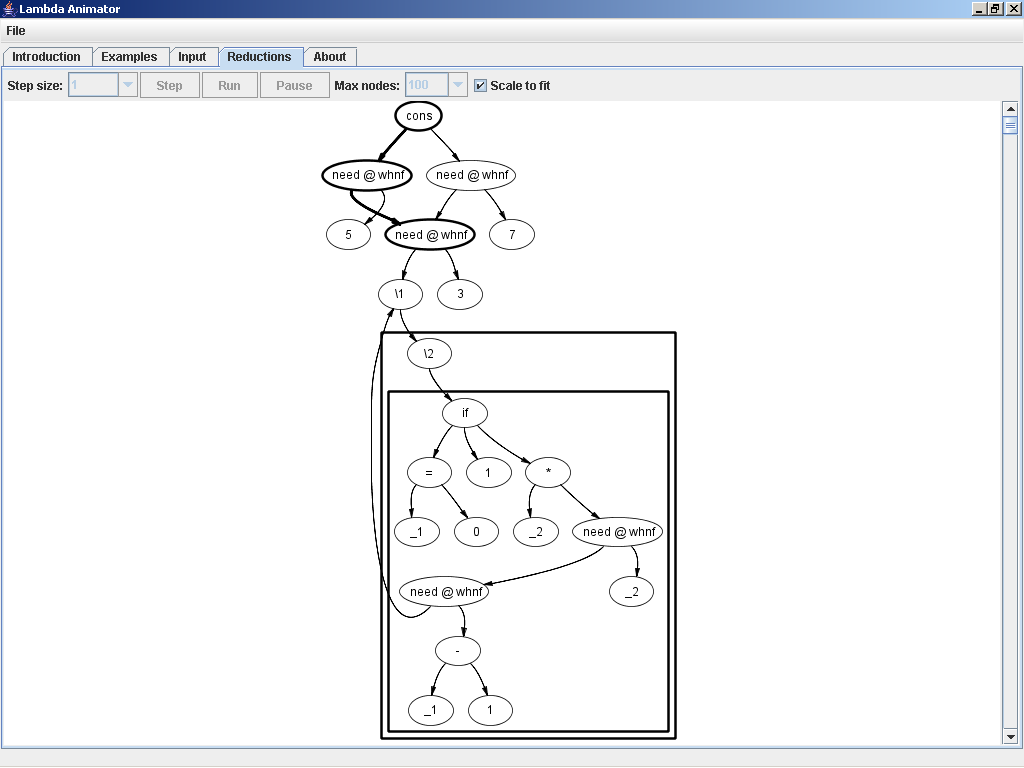
\includegraphics[scale=0.1]{../images/lambdaAnimator.png}
% 	\caption{Screenshot of the Lambda Annimator tool}
% 	\label{fig:images_lambdaAnimator}
% \end{figure}

The Animator does not seem very smooth and does not produce graphs that are
neither pretty nor especially visually informative. It uses extremely simple
graphics and does not fulfill our ``pretty'' criteria. The implementation in
the form of a Java applet does have some advantages in terms of easy access to
the tool.

It can give an reasonable overview when the lambda terms are not to complex.
In figure \ref{fig:images_lambdaAnimatorReduction} there is an example of a
simple $\beta$-reduction.
% \begin{figure}[!htbp]
% 	\centering
% 		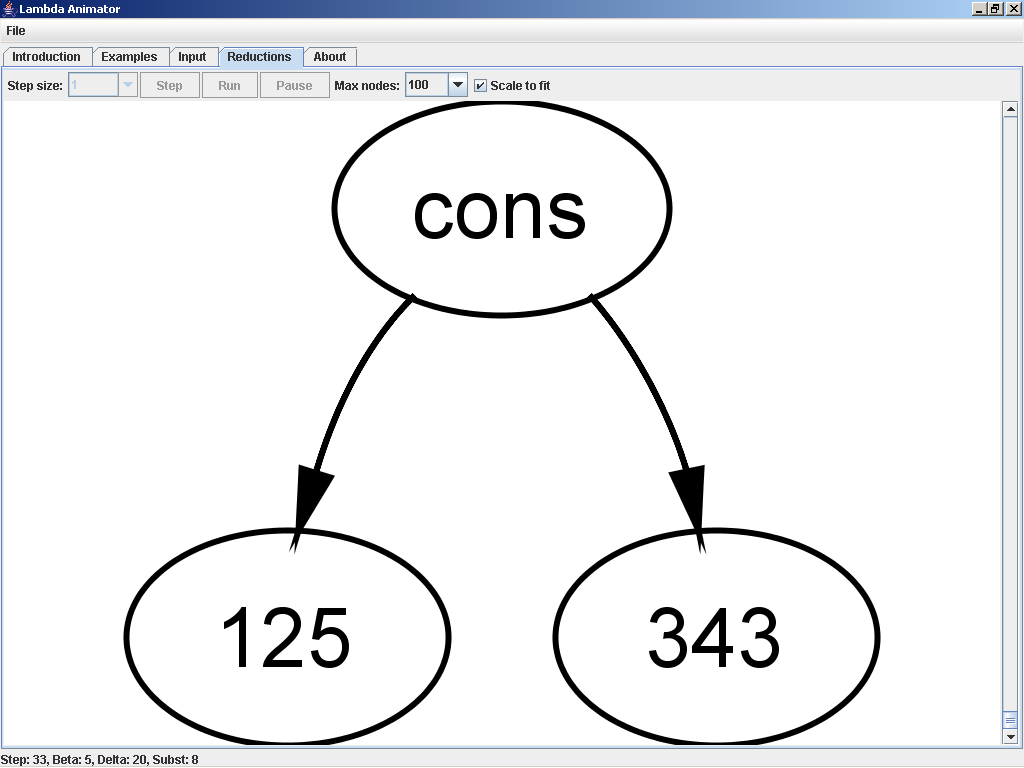
\includegraphics[scale=0.25]{../images/lambdaAnimatorReduction.png}
% 	\caption{Example of a simple $\beta$-reduction in the Lambda Animator}
% 	\label{fig:images_lambdaAnimatorReduction}
% \end{figure}

When you are dealing with more complex lambda terms it very easy gets chaotic.
In figure \ref{fig:images_lambdaAnimatorComplex} there is another example, in
which one can see that the informativeness seems to drastically degrade when
the term complexity is increasing.
% \begin{figure}[!htbp]
% 	\centering
% 		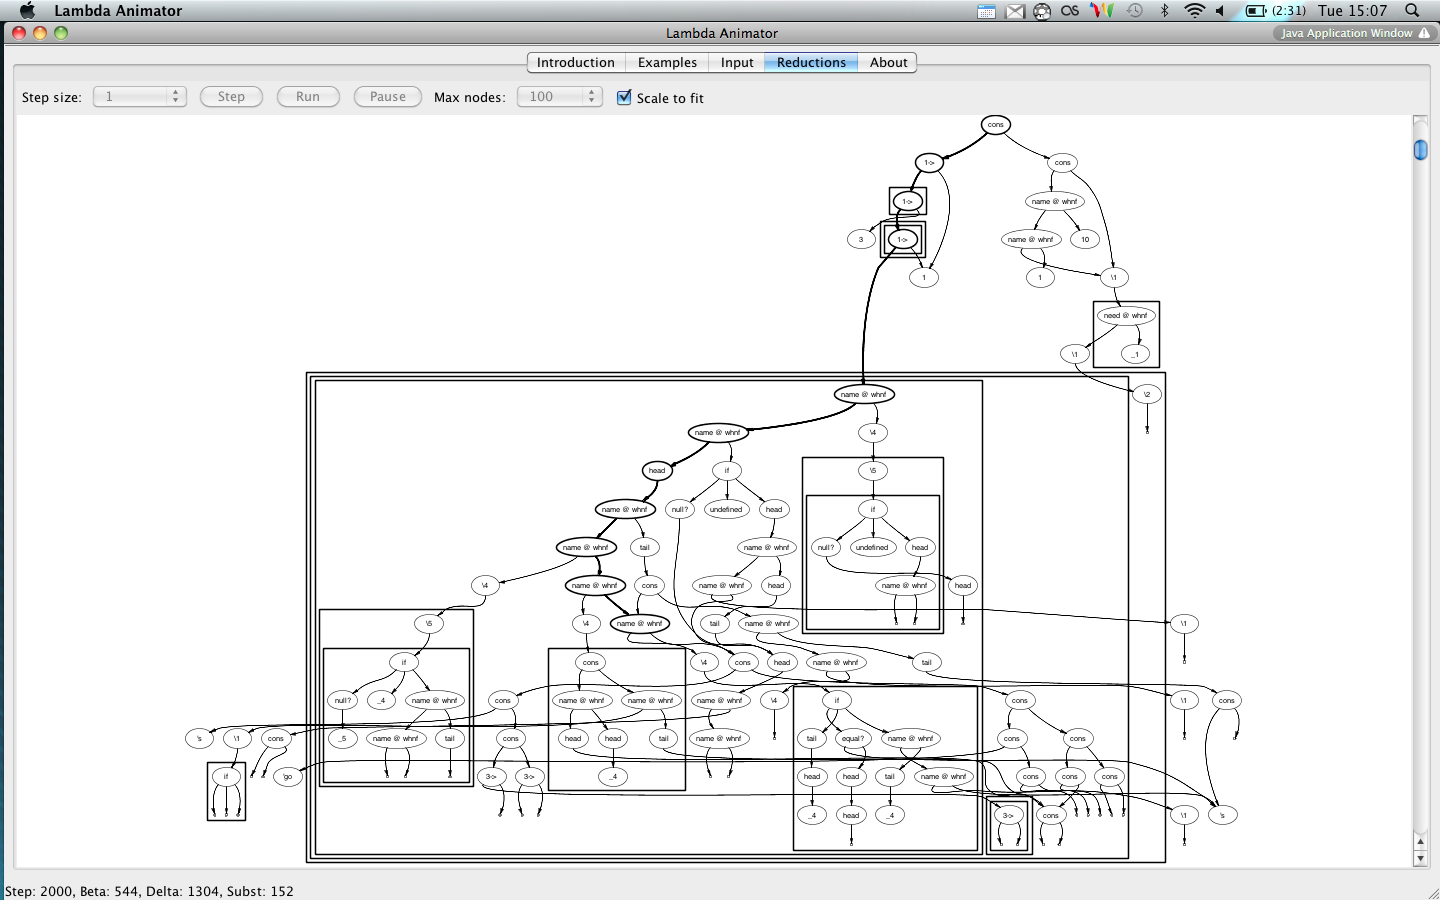
\includegraphics[scale=0.25]{../images/lambdaAnimatorComplex.png}
% 	\caption{Complex example in the Lambda Animator}
% 	\label{fig:images_lambdaAnimatorComplex}
% \end{figure}